\documentclass[10pt,a4paper]{article}
\usepackage{amsmath,amssymb,amsthm,graphicx}
\usepackage{amsfonts,amssymb,amsmath,amsthm}
\usepackage{latexsym}
\usepackage{calc}
\usepackage{url}
\usepackage{thmtools}
\usepackage{thm-restate}
\usepackage{hyperref}
\usepackage[capitalise, nameinlink]{cleveref}
\usepackage{algorithm}
\usepackage{algorithmicx}
\usepackage{algpseudocode}
\usepackage{color}
\usepackage{graphicx}
\usepackage{enumitem}
\setcounter{MaxMatrixCols}{15}

%%% Basic notation
\newcommand{\N}{\mathbb{N}}
\newcommand{\Q}{\mathbb{Q}}
\newcommand{\R}{\mathbb{R}}
\newcommand{\Z}{\mathbb{Z}}
\newcommand{\F}{\mathbb{F}}
\newcommand{\zero}{\mathbf{0}}
\newcommand{\Id}{\mathbf{I}}
\newcommand{\vecu}{\vec{u}}
\newcommand{\Acal}{\mathcal{A}}
\newcommand{\Ccal}{\mathcal{C}}
\newcommand{\Hcal}{\mathcal{H}}
\newcommand{\Lcal}{\mathcal{L}}
\newcommand{\Pcal}{\mathcal{P}}
\newcommand{\Rcal}{\mathcal{R}}
\newcommand{\Mcal}{\mathcal{M}}
\newcommand{\Kcal}{\mathcal{K}}
\newcommand{\M}{\mathcal{M}}
\newcommand{\Scal}{\mathcal{S}}
\newcommand{\Tcal}{\mathcal{T}}
\newcommand{\Fcal}{\mathcal{F}}
\newcommand{\Gcal}{\mathcal{G}}
\newcommand{\Xcal}{\mathcal{X}}
\newcommand{\Tr}{\mathrm{Tr}}
\newcommand{\OR}{\mathrm{OR}}
\newcommand{\MAJ}{\mathrm{MAJ}}
\newcommand{\atoms}{\mathrm{atoms}}
\newcommand{\symvec}{\mathrm{symvec}}
\newcommand{\symmat}{\mathrm{Sym}}
\newcommand{\MINCUT}{\mathrm{MINCUT}}
\newcommand{\ARGMINCUT}{\mathrm{ARGMINCUT}}
\newcommand{\CON}{\mathrm{CON}}
\newcommand{\THRESH}{\mathrm{THRESHOLD}}
\newcommand{\Contract}{\mathrm{Contract}}
\newcommand{\lin}{\mathrm{lin}}
\newcommand{\cut}{\mathrm{cut}}
\newcommand{\ind}{\mathrm{ind}}
\newcommand{\diag}{\mathrm{diag}}
\newcommand{\rmin}{\mathrm{in}}
\newcommand{\rmout}{\mathrm{out}}
\newcommand{\IP}{\mathrm{IP}}
\newcommand{\PARITY}{\mathrm{PARITY}}
\newcommand{\upto}{\mathbin{:}}
\DeclareMathOperator*{\argmin}{argmin}
\newcommand{\polylog}{\mathrm{polylog}}
\newcommand{\zeros}{\mathrm{zeros}}
\newcommand{\ones}{\mathrm{ones}}
\newcommand{\rmvec}{\mathrm{vec}}
\newcommand{\rmmat}{\mathrm{mat}}
\newcommand{\laspan}{\mathrm{span}}
\newcommand{\cross}{\mathrm{overlap}}
\newcommand{\shore}{\mathrm{shore}}
\newcommand{\edges}{\mathrm{cutedges}}
\newcommand{\coisa}{weighted biadjacency matrix }
\newcommand{\card}[1]{|#1|}
\newcommand{\len}[1]{l(#1)}
\newcommand{\floor}[1]{\lfloor #1 \rfloor}
\newcommand{\ceil}[1]{\left\lceil #1 \right\rceil}
\newcommand{\pair}[2]{\langle #1,#2 \rangle}
\newcommand{\triple}[3]{\langle #1,#2,#3 \rangle}
\def\01{\{0,1\}}

\newcommand{\ith}{i^{\scriptsize \mbox{{\rm th}}}}
\newcommand{\jth}{j^{\scriptsize \mbox{{\rm th}}}}
\newcommand{\kth}{k^{\scriptsize \mbox{{\rm th}}}}
\newcommand{\ellth}{\ell^{\scriptsize \mbox{{\rm th}}}}

\newcommand{\cd}{\mathrm{cdim}}
\newcommand{\sep}{\mathrm{sep}}
\newcommand{\mer}{\mathrm{mer}}

\DeclareMathOperator*{\argmax}{arg\,max}

\newcommand{\norm}[1]{\|#1\|}


\newcommand{\troy}[1]{\textcolor{red}{#1}}

% new commands Simon
\newcommand{\tO}{\tilde O}
\newcommand{\Ecal}{\mathcal{E}}
\newcommand{\simon}[1]{\textcolor{blue}{Simon: #1}}
\declaretheorem[name=Theorem,numberwithin=section]{thm}

\newcommand{\bra}[1]{\langle#1|}
\newcommand{\ket}[1]{|#1\rangle}
\newcommand{\bigket}[1]{\big|#1\big\rangle}
\newcommand{\braket}[2]{\langle#1, #2\rangle}
\newcommand{\rk}{\mathrm{rk}}
\newcommand{\I}{\mathcal{I}}
\newcommand{\1}{\mathbf{1}}


\newtheorem{theorem}{Theorem}
\newtheorem{question}[theorem]{Question}
\newtheorem{lemma}[theorem]{Lemma}
\newtheorem{corollary}[theorem]{Corollary}
\newtheorem{proposition}[theorem]{Proposition}
\newtheorem{remark}[theorem]{Remark}
\newtheorem{example}[theorem]{Example}
\newtheorem{claim}[theorem]{Claim}
\newtheorem{fact}[theorem]{Fact}
\newtheorem{hypothesis}[theorem]{Hypothesis}

\theoremstyle{definition}
\newtheorem{exercise}[theorem]{Exercise}
\newtheorem{problem}[theorem]{Problem}
\newtheorem{definition}[theorem]{Definition}
\title{Quantum minimum-cut query lower bounds for weighted graph input models}
\author{Simon Apers, Troy Lee}
\date{doi:10.4230/LIPIcs.CCC.2021.28; CC BY-NC-SA4.0}
\begin{document}
\maketitle
\noindent\textit{Editorial note.} Original authors: Simon Apers and Troy Lee. arXiv:2011.09823v3, 2021-05-24; accepted CCC2021.\par\medskip
\noindent\textit{Editorial note.} License: CC BY-NC-SA4.0. Noncommercial research adaptation; attribution and share-alike retained.\par\medskip
\noindent\textit{Editorial note.} License terms: https://creativecommons.org/licenses/by-nc-sa/4.0/\par\medskip
\noindent\textit{Editorial note.} Faithful editable selection of author arXiv:2011.09823v3 (2021-05-24), CC BY-NC-SA4.0, for noncommercial research with attribution and share-alike retained. The complete independent Section5 lower-bound family, Theorems35,37,40, is grouped as one item across query models and edge-weight regimes, retaining exact integer/divisibility/error promises, both cut-weight and cut-shore tasks, graph constructions, oracle simulations, local claims and proofs. Exact credited connectivity/counting facts33--34, graph definitions and quantum input-oracle models are retained. Original adjacency-gadget PDF and full bibliography retained. Query/time-upper-bound references are presented explicitly by original Theorem21/Section4 numbers; counters resume their original numbers. Original author mathematics is not corrected or supplemented. No upper-algorithm technical by-product is counted as a separate result.\par\medskip
\noindent\textit{Allowed standard prerequisites (editorial).}\begin{itemize}
\item Connectivity query lower bounds. Exact original Theorem33 [DHHM06] retained as prior context.
\item Approximate-degree counting bound and quantum query composition. Exact original Theorem34 [NW99] and composition citations [HLS07,Rei11a] retained, without recursively reproducing prior literature.
\end{itemize}\medskip
\setcounter{section}{1}
\section{Preliminaries}
For a natural number $n \ge 1$ we let $[n] = \{1, \ldots, n\}$.  For a real number $x$ we let $\lfloor x \rceil$ denote the closest integer to $x$.

\subsection{Graph basics and notation}
Let $V$ be a finite set and $V^{(2)}$ the set of all subsets of $V$ of cardinality $2$.  We represent a weighted undirected 
graph as a pair $G = (V,w)$ where $w: V^{(2)} \rightarrow \R$ is a non-negative function.  We let $V(G)$ be the vertex set of a graph $G$ and 
$E(G) = \{ e \in V^{(2)}: w(e) > 0\}$ be the set of edges of $G$.  We extend the weight function to sets $S \subseteq V^{(2)}$ by $w(S) = \sum_{e \in S} w(e)$.
We say that $G$ is \emph{simple} if $w: V^{(2)} \rightarrow \{0,1\}$ and in this case also denote $G$ as $G = (V,E)$, where $E$ is the set of edges.  We call the 
ratio of the largest edge weight of $G$ to the smallest the \emph{edge-weight ratio} of $G$.


For a subset $X \subseteq V$ we use the shorthand $\overline{X} = V \setminus X$, and we say $X$ is \emph{non-trivial} if $\emptyset \ne X \subsetneq V$.  
For disjoint sets $X,Y \subseteq V$ we use $E(X,Y)$ for the set of edges with one endpoint in $X$ and one endpoint in $Y$.
For a non-trivial set $X$, let $\Delta_G(X) = \{ \{i,j\} \in E(G) : i \in X, j \in \overline{X}\}$ be the set of edges 
of $G$ with one endpoint in $X$ and one endpoint in $\overline{X}$.  A \emph{cut} of $G$ is a set of the form $\Delta_G(X)$ for some non-trivial 
set $X$.  We call $X$ and $\overline{X}$ the \emph{shores} of the cut $\Delta_G(X)$.  We call a cut of the form $\Delta_G(\{u\})$ a \emph{star} cut, and refer 
to all other cuts as \emph{non-star} cuts.  The \emph{weight} of a cut $S$ is $w(S)$, which in the 
case of a simple graph equals $|S|$.  We let $\lambda(G) = \min_{\emptyset \ne X \subsetneq V} w(\Delta_G(X))$ be the minimum weight of a cut in $G$.  
We call a cut realizing this bound a \emph{minimum cut}.  We call a cut $\Delta_G(X)$ satisfying $w(\Delta_G(X)) \le \alpha \lambda(G)$ an $\alpha$-near minimum cut. 
In the case where $G$ is simple we call $\lambda(G)$ the \emph{edge connectivity} of $G$.  
We will only use the term edge connectivity in the context of unweighted graphs.



\setcounter{subsection}{2}
\subsection{Quantum query and computational models}
For general background on the quantum query model we refer the reader to \cite{HLS07}. 
Here we restrict ourselves to describing the quantum 
implementation of the input oracles in the adjacency matrix and adjacency array models.

In the adjacency matrix model, on input a weighted graph $G = (V,w)$, classically one can query any $\{u,v\} \in V^{(2)}$ and receive the answer 
$w(\{u,v\})$.  We now describe how to model this by a quantum query.  We will assume that the 
edge weights are given as binary decimal numbers with $M_1$ bits before the decimal and $M_2$ bits after the decimal for a total of $M = M_1 + M_2$ bits.  
The state of the quantum query 
algorithm will have three registers, a query register, an answer register, and a workspace register.  The 
state of the algorithm will in general be in a superposition of the basis states $|\{u,v\} \rangle |b \rangle | a \rangle$ where $\{u,v\} \in V^{(2)}, b \in \{0,1\}^M$ 
and $a \in \Acal$ for an arbitrary finite set $\Acal$.  
On input graph $G = (V,w)$, the input oracle $\mathsf{O}_G$ acts on a basis state $|\{u,v\} \rangle |b \rangle | a \rangle$ as
\[
\mathsf{O}_G |\{u,v\} \rangle |b \rangle | a \rangle = |\{u,v\} \rangle |b \oplus w(\{u,v\}) \rangle | a \rangle \enspace.
\]
 
In the adjacency array model, on input a weighted $n$-vertex graph $G = (V,w)$ one can make two types of queries.  In the first type, one can query a vertex $v \in V$ and receive its degree $\deg(v)$.
The second type is specified by a family of functions $\{f_v : [\deg(v)] \rightarrow V\}_{v \in V}$ such that $f_v(i)$ corresponds to the $\ith$ neighbor of vertex $v$ (according to some arbitrary but fixed ordering).  
A query consists of a pair $(v,i)$ for $i \in [\deg(v)]$ and the returned answer is the pair
$(f_v(i), w(\{v,f_v(i)\}))$.  In this paper we will only 
need to model the second type of query quantumly.  This is because our upper bounds are larger than $n$ so we can let the algorithm classically 
query all degrees at the start of the algorithm, and in our lower bound on the query complexity of edge connectivity for weighted graphs we assume the 
algorithm already knows the degree of every vertex.  
The state of the quantum query algorithm will again have a query register, an answer register, and a workspace register, with the state of the algorithm 
in general being in a superposition of the basis states $|(v,i)\rangle |x \rangle |b \rangle | a \rangle$ where $v \in V, i \in [\deg(v)], x \in \{0,\ldots, n-1\}, b \in \{0,1\}^M$, 
and $a \in \Acal$ for an arbitrary finite set $\Acal$.  We further let $\tau : V \rightarrow \{0,1,\ldots, n-1\}$ be a bijection where $|V| = n$.  Then the input oracle $\mathsf{O}_G$ acts on a basis state in the following way:
\[
\mathsf{O}_G |(v,i)\rangle |x \rangle |b \rangle | a \rangle = |(v,i) \rangle |x + \tau(f_v(i)) \bmod n \rangle |b \oplus w(\{v,f_v(i)\}) \rangle | a \rangle \enspace.
\]

In Section~4 of the source we will further show that our query algorithms can be implemented in a time efficient manner.  We analyze the time complexity in terms of the standard quantum circuit model augmented with two types of oracles.  
One is the oracle for the input, either in the adjacency matrix or array model, and the second is an oracle to a classical memory of $\tO(n)$ bits.  The latter corresponds to a \emph{quantum random-access-memory} or \emph{QRAM}.  We further assume that 
we can classically update a value in this $\tO(n)$ bit classical memory in time $\tO(1)$.  
The assumption of QRAM access is also required for the time efficiency of the sparsifier construction in \cite{AdW19} which our algorithms build on, and in fact is a necessary (but sometimes inexplicit) assumption in the time analysis of many quantum algorithms for graph problems, e.g.~\cite{DHHM06,Amb06,B13}.


\setcounter{section}{4}
\setcounter{theorem}{32}
\section{Lower bounds} \label{sec:lower-bounds}
In this section we present lower bounds on the complexity of edge connectivity and weighted minimum cut.

First we describe some existing lower bounds for the case of simple graphs.
Let $\CON_n$ be the problem of deciding if an input \emph{simple} graph on $n$ vertices is connected or not.  This is a special case of edge connectivity, where one wants 
to decide if the edge connectivity is zero or positive.  D\"{u}rr, Heiligman, H{\o}yer and Mhalla \cite{DHHM06} proved the following quantum query lower bounds on the complexity of $\CON_n$.
\begin{theorem}[\cite{DHHM06}]
\label{thm:durr_lower}
The bounded-error quantum query complexity of $\CON_n$ is $\Theta(n^{3/2})$ in the adjacency matrix model and 
$\Theta(n)$ in the adjacency array model.  
\end{theorem}
\noindent
This theorem shows that, in the adjacency matrix model, Theorem~21 of the source is tight up to polylogarithmic factors for simple graphs.  For the adjacency array model 
there is still a gap between the $\Omega(n)$ lower bound from \cref{thm:durr_lower} and the $\tilde O(\sqrt{mn})$ upper bound for simple graphs given by Theorem~21 of the source.

For the minimum cut problem in a weighted graph we prove separate and distinct lower bounds for the adjacency matrix model and the adjacency array model.
All our lower bounds essentially follow by forcing the algorithm to solve a counting problem in order to compute the weight of a minimum cut.
We then use the following theorem by Nayak and Wu that gives a lower bound on the quantum query complexity of exact counting.

\begin{theorem}[{\cite[Corollary 1.2]{NW99}}]
\label{thm:thresh}
Let $k,N \in \N$ with $2k+1 \le N$.  Assume query access to $x \in \{0,1\}^N$ with the promise that $|x| = k+1$ or $|x| = k-1$.  Any quantum algorithm that correctly decides whether $|x| = k+1$ or $|x| = k-1$ with probability at least $2/3$ must make $\Omega(\sqrt{N k})$ queries.
\end{theorem}

\subsection{Adjacency matrix model}

In the adjacency matrix model we show that for any integer $1 \le \tau \le (\floor{n/2}-1)/2$, in the worst case $\Omega( n^{3/2} \sqrt{\tau})$ adjacency matrix queries are needed to compute the weight of a minimum cut of a graph with edge weights in 
$\{1,\tau\}$.
This matches the upper bound in Theorem~21 of the source, and hence settles the quantum query complexity of weighted minimum cut in the adjacency matrix model.
For $\tau = 1$ this reproduces the aforementioned $\Omega(n^{3/2})$ bound which follows from \cite{DHHM06}.


\begin{theorem}
\label{thm:lower}
Let $n,\tau \in \N$ satisfy $1 \le \tau \le (\floor{n/2}-1)/2$.  There is a family of $n$-vertex graphs $\Gcal$ all of which have edge weights in $\{0,1,\tau\}$ 
such that any quantum algorithm that for every graph $G \in \Gcal$ computes with probability at least $2/3$ the weight of a minimum cut in $G$ must make 
$\Omega(n^{3/2}\sqrt{\tau})$ queries in the adjacency matrix model.  Similarly, any quantum algorithm that for every graph $G \in \Gcal$ computes with 
probability at least $2/3$ the shores $(X,\overline{X})$ of a cut realizing the minimum weight must make $\Omega(n^{3/2}\sqrt{\tau})$ queries in the adjacency matrix model.
\end{theorem}


\begin{proof}
Let $V$ be an $n$-element set and partition $V$ into disjoint sets $V = V_0 \sqcup V_1$ where $|V_0| = \floor{n/2}$, $|V_1| = \ceil{n/2}$.  Choose a distinguished vertex $v_0 \in V_0$, and let $V_0' = V_0 \setminus \{v_0\}$. 
Let $N = |V_0' \times V_1|$ and let $g : V_0' \times V_1 \rightarrow [N]$ be a bijection.  For every $x \in \{0,1\}^N$ we define a weighted graph $G_x = (V,w_x)$ where
\begin{itemize}
\item
$w_x(\{u,v\}) = \tau$ if $u,v \in V_0$ or $u,v \in V_1$,
\item
$w_x(\{u,v\}) = x(g(\{u,v\}))$ if $(u \in V_0', v \in V_1)$ or $(u \in V_1, v \in V_0')$,
\item
$w_x(\{u,v\}) = 0$ otherwise.
\end{itemize}
Let $k = \tau (\floor{n/2}- 1)$.  In the following $\Delta_{G_x}(\cdot)$ will always be with respect to $G_x$ and we drop the subscript.
For any $x$ it holds that $w_x(\Delta(V_0)) = |x|$ and $w_x(\Delta(\{v_0\})) = k$.
Now consider any $x$ and a subset $\emptyset \neq Y \subsetneq V$ different from $V_0$ or $V_1$.  We can prove that $w_x(\Delta(Y)) \ge k$.  To this end note that either 
$\emptyset \neq Y \cap V_0 \subsetneq V_0$ or $\emptyset \neq Y \cap V_1 \subsetneq V_1$.  First assume that the former is the case.  Then
\[
w_x(\Delta(Y))
= \sum_{u \in Y, v \notin Y} w_x(\{u,v\})
\ge \sum_{u \in Y \cap V_0, v \in V_0 \backslash Y} w_x(\{u,v\})
\ge k,
\]
as $k$ is the weight of a minimum cut in the complete weighted graph over $\floor{n/2}$ nodes with all edge weights $\tau$.  If instead $\emptyset \neq Y \cap V_1 \subsetneq V_1$ 
then a similar argument shows that $w_x(\Delta(Y)) \ge \tau (\ceil{n/2}-1) \ge k$.

Thus if $|x| < k$ then $\Delta(V_0)$ will be the unique minimum cut of $G_x$, and the weight of a minimum cut in $G_x$ will be $w_x(\Delta(V_0)) = |x|$. On the other hand, if 
$|x| > k$ then the weight of a minimum cut in $G_x$ will be $k$, which is realized by the star cut $\Delta(\{v_0\})$ (and potentially other cuts in $G_x$) but 
not by $\Delta(V_0)$ as $w_x(\Delta(V_0)) = |x| > k$.

Let $\Scal = \{x \in \{0,1\}^N : |x| \in \{k-1,k+1\} \}$ and $\Gcal = \{G_x : x \in \Scal\}$.  
Suppose there was a $T$ query algorithm in the adjacency matrix model that for any $G_x \in \Gcal$ with probability at least $2/3$ output the weight of a minimum cut in $G_x$.
If the output is $<k$ then we know that $|x| = k-1$ and if the output is $k$ then we know that $|x| = k+1$.  Moreover, any query to the adjacency matrix of $G_x$ can be simulated 
by a query to $x$, thus such an algorithm gives a $T$ query algorithm to determine if $|x| = k-1$ or $|x| = k+1$ when we are promised one of these is the case.  Since $\tau \le (\floor{n/2}-1)/2$ 
we have $2k+1 \le N$ and therefore we may apply Theorem \ref{thm:thresh} to obtain $T \in \Omega(\sqrt{N k}) = \Omega(n^{3/2}\sqrt{\tau})$.

Similarly, a $T$ query algorithm in the adjacency matrix model that for any $G_x \in \Gcal$ with probability at least $2/3$ outputs the shores of a cut realizing the minimum weight 
also implies a $T$ query algorithm to determine if $|x| = k-1$ or $|x| = k+1$.  In this case, if $|x| = k-1$ then the output must be $(V_0, \overline{V}_0)$ as these are the shores of the unique 
minimum cut in $G_x$.  On the other hand, if $|x| = k+1$ then $(V_0, \overline{V}_0)$ is not a correct output.  Thus the output of the algorithm lets us determine with probability at least $2/3$ if 
$|x| = k-1$ or $|x| = k+1$ and we again have $T \in \Omega(\sqrt{N k}) = \Omega(n^{3/2}\sqrt{\tau})$.
\end{proof}

\subsection{Adjacency array model}
Given adjacency array access to a graph with edge-weight ratio $\tau$, we showed an upper bound of $\tO(\sqrt{m n \tau})$ on the quantum query complexity of computing the weight of a minimum cut.
In this section we prove two distinct lower bounds, each of which is tight in a specific regime.
First we show that for any $\tau > 1$ there exists a family of dense graphs on $n$ vertices with edge-weight ratio $\tau$ for which computing the weight of a minimum cut requires $\Omega(n^{3/2})$ queries to the adjacency array.
This shows that the adjacency array upper bound of Theorem~21 of the source is tight for dense weighted graphs with constant (but non-unit) edge-weight ratio.
Secondly and using a different approach, for any $1 \leq \tau \in O(n)$ we prove an $\Omega(\tau n)$ lower bound for a family of dense graphs with edge-weight ratio $\tau$.
This shows that we cannot get a quantum speedup when $\tau \in \Omega(n)$.

\subsubsection{Constant edge-weight ratio}

For the first bound we first need a claim about the minimum cuts of a complete weighted bipartite graph.
\begin{claim}
\label{clm:complete_bipartite}
Let $n \ge 8$ be a multiple of $4$ and $G=(L \sqcup R,w)$ be a weighted bipartite graph with bipartition $L,R$ where $|L| = 3n/4, |R| = n/4$. Further suppose that 
for every $x \in L, y \in R$ it holds that $w(\{x,y\}) \ge 1$.   Then any cut of $G$ that is not of the form $\Delta_G(\{x\})$ for $x \in L$ has weight at least $n/2$.  
\end{claim}

\begin{proof}
First consider a star cut $\Delta_G(\{y\})$ for $y \in R$.  This has weight at least $3n/4$, since this is the degree of $y$ and all edges have weight at least 1.  

It now remains to show the claim holds for non-star cuts.  Consider a general non-star cut with shore $X \cup Y$ with $X \subseteq L, Y \subseteq R$.  Let 
$k = |X|, \ell = |Y|$.  As it is a non-star cut we have $k + \ell \ge 2$.  By complementing as needed we may also assume that $k \le 3n/8$.  We also have 
the obvious constraints that $\ell \le n/4$ and $k,\ell \ge 0$.  

As $G$ is a complete weighted bipartite graph with every edge weight at least one we have
\[
w(\Delta_G(X \cup Y)) \ge k(n/4-\ell) + \ell(3n/4-k) \enspace .
\]
As $k \le 3n/8$ the term $\ell (3n/4-k)$ is greater than $n/2$ whenever $\ell \ge 2$.  Thus we can focus on $\ell \in \{0,1\}$.  
If $\ell=0$ then $k\ge 2$ and so the weight of the cut is at least $k(n/4)=n/2$ as desired.  If $\ell = 1$ then the weight of the 
cut is $k(n/4-1) + 3n/4-k$ which is always at least $3n/4$ as long as $n \ge 8$.  
\end{proof}

This claim means that if $\min_{x \in L} w(\Delta_G(\{x\})) < n/2$ then this value will be the weight of a minimum cut in $G$.  
We can leverage this to show a lower bound as follows.
In the next proof, for a function $f: \{0,1\}^n \rightarrow \{0,1\}$ we will use $Q_{1/3}(f)$ to denote the quantum query complexity of computing $f$ with error at most $1/3$.

\begin{theorem}
\label{thm:adjlower2}
Let $n \ge 8$ be a multiple of $4$ and $0 < \varepsilon \le 1$.  There is a family of $n$-vertex graphs $\Gcal$ all of which have edge weights in $\{1,1+\varepsilon\}$ 
such that any quantum algorithm that for every graph $G \in \Gcal$ computes with probability at least $2/3$ the weight of a minimum cut in $G$ must make 
$\Omega(n^{3/2})$ queries in the adjacency array model.  Similarly, any quantum algorithm that for every graph $G \in \Gcal$ computes with 
probability at least $2/3$ the shores $(X,\overline{X})$ of a cut realizing the minimum weight must make $\Omega(n^{3/2})$ queries in the adjacency array model.
\end{theorem}


\begin{proof}
Let $X =\{x \in \{0,1\}^{n/4}: |x| = \floor{n/8}-1\}$ and $Y =\{y \in \{0,1\}^{n/4}: |y| = \floor{n/8}+1\}$.  For every 
$x = (x^{(1)}, \ldots, x^{(3n/4)}) \in (X \cup Y)^{3n/4}$ we associate a bipartite graph $G_x = (L \sqcup R, w_x)$ 
where $L = \{1, \ldots, 3n/4\}, R = \{3n/4+1, \ldots, n\}$ and $w_x(\{i,j\}) = 1+ \varepsilon \cdot x^{(i)}(j-3n/4)$ for every $i \in L, j \in R$.  We set $\Gcal = \{G_x : x \in (X \cup Y)^{3n/4}\}$.

Define the function $g: X \cup Y \rightarrow \{0,1\}$ where $g(x) = 0$ iff $x \in X$.  We have $Q_{1/3}(g) \in \Omega(n)$ by \cref{thm:thresh}.  
Let $f : \{0,1\}^{3n/4} \rightarrow \{0,1\}$ be the AND function, for which $Q_{1/3}(f) \in \Omega(\sqrt{n})$.  By the composition theorem for quantum query complexity \cite{HLS07,Rei11a}, 
we have $Q_{1/3}(h) \in \Omega(n^{3/2})$ for the composed function $h = f \circ g^{3n/4}$.   

Let $x = (x^{(1)}, \ldots, x^{(3n/4)}) \in (X \cup Y)^{3n/4}$.  If $h(x) = 1$ then $x^{(i)} \in Y$ for all $i \in [3n/4]$ and the weight of the star cut $\Delta_{G_x}(\{i\}) = n/4 + \varepsilon \cdot(\floor{n/8}+1)$.  
As $\varepsilon \le 1$ this will be the weight of a minimum cut in $G_x$ by \cref{clm:complete_bipartite}.  On the other hand if $h(x) = 0$ then some $x^{(i)} \in X$ and 
$\Delta_{G_x}(\{i\}) = n/4 + \varepsilon \cdot(\floor{n/8}-1)$ and this will be the weight of a minimum cut of $G_x$.
Thus computing the weight of a minimum cut of $G_x$ lets us evaluate $h(x)$.  Further, given oracle access to $x$ we can 
simulate queries to $G_x$ in the adjacency array model.  Let $A_x$ be a $3n/4$-by-$n/4$ matrix whose $\ith$ row is the vector $1+ \varepsilon x^{(i)}$.  Then the vertical concatenation of $A$ with 
$A^T$ is a valid adjacency array for $G_x$.  To a degree query on vertex $i$ we simply answer $n/4$ if $1 \le 3n/4$ and $3n/4$ if $3n/4+1 \le i \le n$.  We can also answer 
a query to the name and weight of the $\jth$ neighbor of $i$ with one query to $x$.  This shows that the (1/3)-error quantum query complexity of computing the weight of 
a minimum cut on graphs in $\Gcal$ in the adjacency array model is at least $Q_{1/3}(f \circ g^{3n/4}) \in \Omega(n^{3/2})$.  

Finally, suppose a quantum query algorithm can compute a shore of a minimum cut in $G_x$ with $T$ queries.  We know that this shore must be of the form $\{v\}$ for a vertex $v \in L$.  
Thus with with $O(n)$ more queries the algorithm can classically compute the weight of a 
minimum cut by querying the weight of the neighbors of $v$.  Thus $T + O(n) \in \Omega(n^{3/2})$, which means $T \in \Omega(n^{3/2})$.  This completes the proof.
\end{proof}

\subsubsection{Large edge-weight ratio}
Let $n \in \N$ be a multiple of $4$ and $V$ be a vertex set with $|V| = n$.  Partition $V$ into four sets 
$V_1, V_2, V_3, V_4$.  

Now consider an integer $\tau$ such that $1 \leq \tau \leq 5n/8$ and $\tau n/10$ is an integer.  Fix a set $S$ of 
$\tau n/10$ ``edge disjoint'' quadruples $(u_1, u_2, u_3, u_4) \in V_1 \times V_2 \times V_3 \times V_4$.  By edge disjoint we mean no 
pair of consecutive elements $(u_i, u_{i+1})$ or $(u_4, u_1)$ appears in more than one quadruple. We fix an enumeration 
of $S$ and refer to the vertices in the $\ellth$ quadruple as $u_1^\ell, u_2^\ell, u_3^\ell, u_4^\ell$.  

For every $x \in \{0,1\}^{\tau n/10}$ we define an $n$-vertex weighted graph $G_x = (V,w_x)$ where 
$w_x(\{u,v\}) = \tau$ if $u \ne v \in V_i$ for some $i \in [4]$, and for $\ell \in [\tau n/10]$ we set
\begin{align*}
w_x(\{u^\ell_1,u^\ell_2\}) &= w_x(\{u^\ell_3,u^\ell_4\}) = x_\ell, \\
w_x(\{u^\ell_2,u^\ell_3\}) &= w_x(\{u^\ell_4,u^\ell_1\}) = 1 - x_\ell \enspace.
\end{align*}
Otherwise, $w_x(\{u,v\}) = 0$.  
In words, on each $V_i$ we have a complete graph with all edge weights $\tau$, and for each $\ell \in [\tau n/10]$ we either add unit weight edges
$\{u^\ell_1,u^\ell_2\}, \{u^\ell_3,u^\ell_4\}$ or $\{u^\ell_2,u^\ell_3\},\{u^\ell_4,u^\ell_1\}$ depending on $x_\ell$.  
The construction is depicted in \cref{fig:adj-lower-bound}.

There are a few important points to note about this definition.  First, the edge-weight ratio of $G_x$ is $\tau$.  Second, for any $X$ that nontrivially intersects some $V_i$ we have that 
$w(\Delta_{G_x}(X)) \ge \tau(n/4-1)$.  This means that such an $X$ cannot be the shore of a minimum cut of $G_x$.  Third, by construction 
the degree of every vertex of $G_x$ is independent of $x$.  This means that degree queries to $G_x$ can be trivially answered and give us 
no information about $x$.  

\begin{figure}[htb]
\centering
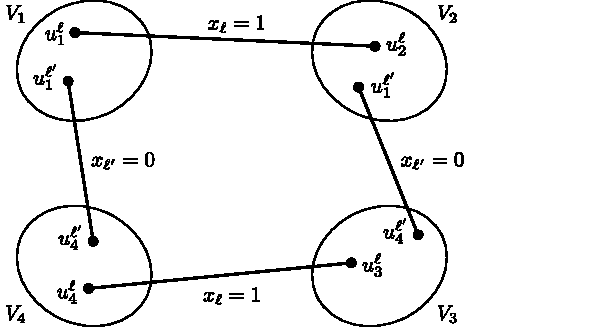
\includegraphics[width=.7\textwidth]{adj-lower-bound.pdf}
\caption{Figure of graph $G_x$.
If $x_\ell = 1$ then we add edges $\{u_1^\ell,u_2^\ell\}$ and $\{u_3^\ell,u_4^\ell\}$.
If $x_\ell = 0$ then we add edges $\{u_2^\ell,u_3^\ell\}$ and $\{u_4^\ell,u_1^\ell\}$.}
\label{fig:adj-lower-bound}
\end{figure}

\begin{lemma} \label{lem:adj-query}
We can simulate a single query to $G_x$ in the adjacency array model using a single query to $x$.
\end{lemma}
\begin{proof}
We first handle degree queries.  This can be answered with no queries to $x$ as the degree of a vertex is independent of $x$.

Now consider a query $(v,k) \in V \times [\deg(v)]$ to which we must answer the name $u$ of the $k$-th neighbor of 
$v$ and the edge weight $w_x(\{u,v\})$.  For clarity of exposition, we assume $v = u_1^t \in V_1$; the other cases are handled similarly.
\begin{itemize}
\item
If $k \leq n/4 - 1$ then return the $k$-th neighbor $u$ of $v$ inside $V_1$ and edge weight $w_x(\{u,v\}) = \tau$.
\item
If $k \ge n/4$ then let $j = k -n/4 +1$.  Letting $\ell$ denote the index of the $\jth$ quadruple of $S$ containing $v$ we query $x_\ell$.
\begin{itemize}
\item
If $x_\ell = 1$ then return neighbor $u^\ell_2$ and edge weight $w(\{v,u^\ell_2\}) = 1$.
\item
If $x_\ell = 0$ then return neighbor $u^\ell_4$ and edge weight $w(\{v,u^\ell_4\}) = 1$.
\end{itemize}
\end{itemize}
In total this takes a single query to $x$, which proves the lemma.
\end{proof}

\noindent
Now we can prove the following lemma.
\begin{lemma} \label{lem:adj-min-cut}
Fix integers $n$ and $\tau$ such that $1 \le \tau \le 5n/8$ and $\tau n/10 \in \N$.
Consider a string $x \in \{0,1\}^{\tau n/10}$ and the corresponding graph $G_x$.
If $|x| < \tau n/20$ then $G_x$ has a unique minimum cut with shores $(X,\overline X) = (V_1 \cup V_2, V_3 \cup V_4)$ and weight $w(\Delta_{G_x}(X)) = 2|x|$.
If $|x| > \tau n/20$ then $G_x$ has a unique minimum cut with shores $(X,\overline X) = (V_1 \cup V_4, V_2 \cup V_3)$ and weight $w(\Delta_{G_x}(X)) = 2(\tau n/10 - |x|)$.
\end{lemma}
\begin{proof}
First consider any cut shore that nontrivially intersects some $V_i$.
Since the subgraph $G_x[V_i]$ induced on $V_i$ is a complete graph with edge weights $\tau$, this implies that such a cut has weight at least $\tau (|V_i|-1) = \tau (n/4-1)$.
Now consider the small set of remaining cut shores that trivially intersect the $V_i$'s.
The weight of each one of these cuts can be easily expressed as a function of the Hamming weight $|x|$ of the input:
\begin{align*}
w(\Delta_{G_x}(V_i))
&= \tau n/10, \\
w(\Delta_{G_x}(V_1 \cup V_3)) &= w(\Delta_{G_x}(V_2 \cup V_4))
= 2 \tau n/10, \\
w(\Delta_{G_x}(V_1 \cup V_2)) &= w(\Delta_{G_x}(V_3 \cup V_4))
= 2 |x|, \\
w(\Delta_{G_x}(V_1 \cup V_4)) &= w(\Delta_{G_x}(V_2 \cup V_3))
= 2 (\tau n/10- |x|).
\end{align*}
It is clear that all minimum weight cuts will be among these cuts, and the lemma easily follows.
\end{proof}

Using this lemma we can prove the following theorem.


\begin{theorem}
\label{thm:adjlowerL}
Let $\tau, n \in \N$ be such that $1 \le \tau \le 5n/8$ and $\tau n/20 \in \N$.
There exists a family of $n$-vertex graphs $\Gcal'$ with $\Omega(n^2)$ edges, all of which have edge weights in $\{1,\tau\}$, such that any quantum algorithm that for every graph $G' \in \Gcal'$ computes with probability at least $2/3$ the weight of a minimum cut in $G'$ must make $\Omega(n \tau)$ queries in the adjacency array model.  Similarly, any quantum algorithm that for every graph $G' \in \Gcal'$ computes with probability at least $2/3$ the shores $(X,\overline{X})$ of a cut realizing the minimum weight must make $\Omega(n \tau)$ queries in the adjacency array model.
\end{theorem}

\begin{proof}
First consider the set of strings $\Xcal \subseteq \{0,1\}^{\tau n/10}$ with Hamming weight
\[
|x|
= \lfloor \tau n/100 \rceil \pm 1
< \tau n/20.
\]
By \cref{lem:adj-min-cut} the graph $G_x$, $x \in \Xcal$, has a unique minimum cut with shores $(V_1 \cup V_2, V_3 \cup V_4)$ and weight $2|x|$.
Now let $\Gcal' = \{G_x : x \in \Xcal\}$ and assume the existence of a quantum algorithm that for every $G_x \in \Gcal'$ computes with probability at least $2/3$ the weight $2|x|$ of a minimum cut in $G'$ with at most $q$ queries to the adjacency array of $G_x$.
By \cref{lem:adj-query} this is equivalent to outputting the Hamming weight $|x|$ with probability at least $2/3$ for any $x \in \Xcal$ while making only $q$ queries to $x$.
Using \cref{thm:thresh} this implies the lower bound $q \in \Omega(\tau n)$.

Next consider the set of strings $\Xcal' \subseteq \{0,1\}^{\tau n/10}$ that have Hamming weight $|x| = \tau n/20 \pm 1$.
By \cref{lem:adj-min-cut} the graph $G_x$, $x \in \Xcal'$, again has a unique minimum cut.
If $|x| = \tau n/20 - 1$ then its shores are $(V_1 \cup V_2, V_3 \cup V_4)$, while if $|x| = \tau n/20 + 1$ then its shores are $(V_1 \cup V_4, V_2 \cup V_3)$.
Now assume that there exists a quantum algorithm that with probability at least $2/3$ returns the shores of a minimum weight cut of $G_x$ with at most $q$ queries to the adjacency array of $G_x$.
By \cref{lem:adj-query} this is equivalent to distinguishing $|x| = \tau n/20 - 1$ from $|x| = \tau n/20 + 1$ with probability at least $2/3$ for any $x \in \Xcal$ while making only $q$ queries to $x$.
Using \cref{thm:thresh} this implies the lower bound $q \in \Omega(\tau n)$.
\end{proof}

\newcommand{\etalchar}[1]{$^{#1}$}
\begin{thebibliography}{BCdWZ99}

\bibitem[AdW20]{AdW19}
Simon Apers and Ronald de~Wolf.
\newblock Quantum speedup for graph sparsification, cut approximation and
  {L}aplacian solving.
\newblock In {\em Proceedings of the 61st Annual Symposium on Foundations of
  Computer Science (FOCS)}, pages 637--648. IEEE, 2020.

\bibitem[A{\v{S}}06]{Amb06}
Andris Ambainis and Robert {\v{S}}palek.
\newblock Quantum algorithms for matching and network flows.
\newblock In {\em Proceedings of the Annual Symposium on Theoretical Aspects of
  Computer Science (STACS)}, pages 172--183. Springer, 2006.

\bibitem[BCdWZ99]{BCWZ99}
Harry Buhrman, Richard Cleve, Ronald de~Wolf, and Christof Zalka.
\newblock Bounds for small-error and zero-error quantum algorithms.
\newblock In {\em Proceedings of the 40th Annual Symposium on Foundations of
  Computer Science (FOCS)}, pages 358--368. IEEE, 1999.

\bibitem[BCJ{\etalchar{+}}13]{B13}
Aleksandrs Belovs, Andrew~M Childs, Stacey Jeffery, Robin Kothari, and
  Fr{\'e}d{\'e}ric Magniez.
\newblock Time-efficient quantum walks for 3-distinctness.
\newblock In {\em International Colloquium on Automata, Languages, and
  Programming}, pages 105--122. Springer, 2013.

\bibitem[BGMP20]{BGMP20}
Arijit Bishnu, Arijit Ghosh, Gopinath Mishra, and Manaswi Paraashar.
\newblock Query complexity of global minimum cut.
\newblock {\em CoRR}, abs/2007.09202, 2020.

\bibitem[BHMT02]{BHMT02}
Gilles Brassard, Peter H{\o}yer, Michele Mosca, and Alain Tapp.
\newblock Quantum amplitude amplification and estimation.
\newblock {\em Quantum computation and quantum information: A millennium
  volume}, 305, 2002.

\bibitem[BK15]{BK15}
Andr{\'{a}}s~A. Bencz{\'{u}}r and David~R. Karger.
\newblock Randomized approximation schemes for cuts and flows in capacitated
  graphs.
\newblock {\em {SIAM} J. Comput.}, 44(2):290--319, 2015.

\bibitem[BLS20]{BLS20}
Nalin Bhardwaj, Antonio~M. Lovett, and Bryce Sandlund.
\newblock A simple algorithm for minimum cuts in near-linear time.
\newblock In {\em Proceedings of the 17th Scandinavian Symposium and Workshops
  on Algorithm Theory (SWAT)}, volume 162 of {\em LIPIcs}, pages 12:1--12:18.
  Schloss Dagstuhl - Leibniz-Zentrum f{\"{u}}r Informatik, 2020.
  
\bibitem[Bot93]{Bot93}
Rodrigo~A. Botafogo.
\newblock Cluster analysis for hypertext systems.
\newblock In {\em Proceedings of the 16th Annual International ACM SIGIR
  Conference on Research and Development in Information Retrieval}, page
  116–125, New York, NY, USA, 1993. Association for Computing Machinery.

\bibitem[BSS12]{BSS12}
Joshua~D. Batson, Daniel~A. Spielman, and Nikhil Srivastava.
\newblock Twice-{R}amanujan sparsifiers.
\newblock {\em {SIAM} J. Comput.}, 41(6):1704--1721, 2012.

\bibitem[DH96]{DH96}
Christoph D{\"{u}}rr and Peter H{\o}yer.
\newblock A quantum algorithm for finding the minimum.
\newblock {\em CoRR}, quant-ph/9607014, 1996.

\bibitem[DHHM06]{DHHM06}
Christoph D{\"{u}}rr, Mark Heiligman, Peter H{\o}yer, and Mehdi Mhalla.
\newblock Quantum query complexity of some graph problems.
\newblock {\em {SIAM} J. Comput.}, 35(6):1310--1328, 2006.

\bibitem[FF62]{FF62}
Lester~R. Ford and Delbert~R. Fulkerson.
\newblock {\em Flows in Networks}.
\newblock Princeton University Press, 1962.

\bibitem[FHHP19]{FHHP19}
Wai~Shing Fung, Ramesh Hariharan, Nicholas J.~A. Harvey, and Debmalya
  Panigrahi.
\newblock A general framework for graph sparsification.
\newblock {\em {SIAM} J. Comput.}, 48(4):1196--1223, 2019.

\bibitem[Gab95]{Gabow95}
Harold~N. Gabow.
\newblock A matroid approach to finding edge connectivity and packing
  arborescences.
\newblock {\em J. Comput. Syst. Sci.}, 50(2):259--273, 1995.

\bibitem[GH61]{GH61}
Ralph~E. Gomory and Te~C. Hu.
\newblock Multi-terminal network flows.
\newblock {\em Journal of the Society for Industrial and Applied Mathematics},
  9(4):551--570, 1961.

\bibitem[GMW20]{GMW20}
Pawe{\l} Gawrychowski, Shay Mozes, and Oren Weimann.
\newblock Minimum cut in ${O}(m \log^2 n)$ time.
\newblock In {\em Proceedings of the 47th International Colloquium on Automata,
  Languages, and Programming (ICALP)}, volume 168 of {\em LIPIcs}, pages
  57:1--57:15. Schloss Dagstuhl - Leibniz-Zentrum f{\"{u}}r Informatik, 2020.
 
\bibitem[GMW21]{GMW20c}
Pawe{\l} Gawrychowski, Shay Mozes, and Oren Weimann.
\newblock A note on a recent algorithm for minimum cut.
\newblock In {\em Symposium on Simplicity in Algorithms (SOSA)}, pages 74--79.
  SIAM, 2021.

\bibitem[Gro97]{Gro97}
Lov Grover.
\newblock Quantum mechanics helps in searching for a needle in a haystack.
\newblock {\em Phys. Rev. Lett.}, 78:325--328, 1997.

\bibitem[HK95]{HK95}
Monika~R. Henzinger and Valerie King.
\newblock Randomized dynamic graph algorithms with polylogarithmic time per
  operation.
\newblock In {\em Proceedings of the 27th annual ACM symposium on Theory of
  computing (STOC)}, pages 519--527, 1995.

\bibitem[HL{\v{S}}07]{HLS07}
Peter H{\o}yer, Troy Lee, and Robert {\v{S}}palek.
\newblock Negative weights make adversaries stronger.
\newblock In {\em Proceedings of the 39th Annual {ACM} Symposium on Theory of
  Computing (STOC)}, pages 526--535. {ACM}, 2007.

\bibitem[HRW20]{HRW20}
Monika~R. Henzinger, Satish Rao, and Di~Wang.
\newblock Local flow partitioning for faster edge connectivity.
\newblock {\em {SIAM} J. Comput.}, 49(1):1--36, 2020.

\bibitem[HW96]{HW96}
Monika~R. Henzinger and David~P. Williamson.
\newblock On the number of small cuts in a graph.
\newblock {\em Inf. Process. Lett.}, 59(1):41--44, 1996.

\bibitem[Kar99]{Karger99}
David~R. Karger.
\newblock Random sampling in cut, flow, and network design problems.
\newblock {\em Mathematics of Operations Research}, 24(2):383--413, 1999.

\bibitem[Kar00]{Karger00}
David~R. Karger.
\newblock Minimum cuts in near-linear time.
\newblock {\em J. {ACM}}, 47(1):46--76, 2000.

\bibitem[KT19]{KT19}
Ken{-}ichi Kawarabayashi and Mikkel Thorup.
\newblock Deterministic edge connectivity in near-linear time.
\newblock {\em J. {ACM}}, 66(1):4:1--4:50, 2019.

\bibitem[Li21]{Li20}
Jason Li.
\newblock Deterministic mincut in almost-linear time.
\newblock In {\em Proceedings of the 53rd annual ACM symposium on Theory of
  computing (STOC)}, 2021.

\bibitem[LST20]{LST20}
On-Hei~S. Lo, Jens~M. Schmidt, and Mikkel Thorup.
\newblock Compact cactus representations of all non-trivial min-cuts.
\newblock {\em Discrete Applied Mathematics}, 2020.

\bibitem[Mat93]{Mat93}
David~W. Matula.
\newblock A linear time 2+epsilon approximation algorithm for edge
  connectivity.
\newblock In Vijaya Ramachandran, editor, {\em Proceedings of the 4th Annual
  {ACM/SIGACT-SIAM} Symposium on Discrete Algorithms (SODA)}, pages 500--504.
  {ACM/SIAM}, 1993.

\bibitem[MN20]{MN20}
Sagnik Mukhopadhyay and Danupon Nanongkai.
\newblock Weighted min-cut: sequential, cut-query, and streaming algorithms.
\newblock In {\em Proceedings of the 52nd Annual ACM SIGACT Symposium on Theory
  of Computing (STOC)}, pages 496--509, 2020.

\bibitem[NI92]{NI92}
Hiroshi Nagamochi and Toshihide Ibaraki.
\newblock Computing edge-connectivity in multigraphs and capacitated graphs.
\newblock {\em {SIAM} J. Discret. Math.}, 5(1):54--66, 1992.

\bibitem[NW99]{NW99}
Ashwin Nayak and Felix Wu.
\newblock The quantum query complexity of approximating the median and related
  statistics.
\newblock In {\em Proceedings of the 31st annual ACM symposium on Theory of
  computing (STOC)}, pages 384--393, 1999.

\bibitem[PQ82]{PQ82}
Jean-Claude Picard and Maurice Queyranne.
\newblock Selected applications of minimum cuts in networks.
\newblock {\em INFOR: Information Systems and Operational Research},
  20(4):394--422, 1982.

\bibitem[Rei11]{Rei11a}
Ben Reichardt.
\newblock Reflections for quantum query algorithms.
\newblock In {\em Proceedings of the 22nd Annual {ACM-SIAM} Symposium on
  Discrete Algorithms (SODA)}, pages 560--569. {SIAM}, 2011.
  
 \bibitem[RSW18]{RSW18}
Aviad Rubinstein, Tselil Schramm, and S.~Matthew Weinberg.
\newblock Computing exact minimum cuts without knowing the graph.
\newblock In {\em Proceedings of the 9th Innovations in Theoretical Computer
  Science Conference (ITCS)}, pages 39:1--39:16. LIPICS, 2018.

\bibitem[TV84]{TV84}
Robert~E. Tarjan and Uzi Vishkin.
\newblock Finding biconnected components and computing tree functions in
  logarithmic parallel time.
\newblock In {\em Proceedings of the 25th Annual Symposium on Foundations of
  Computer Science (FOCS)}, pages 12--20. IEEE, 1984.

\end{thebibliography}
  
%%%%%%%%%%%%%%%%%%%%%%%%%%%%%%%%%%%%%%%%%%%%%%%%%%%%%%%%%%%%%%%%%%%


\end{document}
